\chapter[Curiosidades finais]{Curiosidades finais}
\label{cap-6}
\chaptermark{}
%
\hfill%
\begin{minipage}{10cm}
\begin{flushright}
\rightskip=0.5cm
\textit{``Frase filosófica.''}
\\[0.1cm]
\rightskip=0.5cm
--- Autor cabuloso
\end{flushright}
\end{minipage}

\section{O problema da palavra em \texorpdfstring{$B_n(\mathbb{R}^2)$}{BnR2} -- uma breve introdução}\label{secao o problema da palavra}
	\hspace{12pt} Vamos agora falar mais um pouco sobre o problema da palavra em $B_n$. Mas o que é o problema da palavra? 
	\par\vspace{0.3cm} De modo geral, suponha que nos seja dado um grupo $G$ com apresentação
	\begin{equation*}
	G = \langle x_1, x_2, \dots, x_n| w_1=w_2=\cdots=w_m=1 \rangle
	\end{equation*}
	\par\vspace{0.3cm} sendo $m$ e/ou $n$ não necessariamente finitos. Como vimos anteriormente no Capítulo \ref{cap-grupos-livres}, a partir dessa apresentação qualquer elemento $g$ de $G$ pode ser expresso como uma palavra nos geradores $x_i$ de $G$ e seus inversos. 
	\par\vspace{0.3cm} O problema da palavra consiste em encontrar um método (razoavelmente prático) que nos permita decidir se duas palavras arbitrárias $g_1$ e $g_2$ em $G$ são iguais ou, equivalentemente, dado um elemento $g (=g_1g_2^{-1})$, nos permita decidir se $g=1$, ou seja, trivial.
	\par\vspace{0.3cm} O problema da palavra é um dos problemas fundamentais em Teoria dos Grupos. Infelizmente, não é garantido que tal método sempre exista. Contudo, se existir, dizemos que o problema da palavra é \textit{solúvel} para $G$; do contrário, dizemos que o problema da palavra é \textit{insolúvel} para $G$.  
	\par\vspace{0.3cm} Dissemos que o método deve ser "razoavelmente prático". Bom, isso é algo bem vago e não exatamente uma afirmação matemática. Na verdade, para ser mais preciso, o problema da palavra pertence ao reino da Lógica Matemática ao invés da Teoria dos Grupos. Então, uma primeira investida na direção de uma solução do problema da palavra é tentar deixar claro, matematicamente, o que é possível quando dizemos "razoavelmente prático". Uma boa maneira de fazer isso é olhar para alguns grupos nos quais o problema da palavra é solúvel.
	\begin{theorem}
		\label{problema da palavra soluvel para grupos livres}
		O problema da palavra para um grupo livre é solúvel.
	\end{theorem}
	\begin{proof}
		Seja $F$ um grupo livre em $n$ geradores, $x_1, \dots, x_n$. Um elemento 
		\begin{equation*}
		g = x_{i_1}^{\varepsilon_1}\cdots x_{i_m}^{\varepsilon_m}
		\end{equation*}
		\par\vspace{0.3cm} de $F$ é igual à palavra vazia, $1$, se e somente se podemos eliminar cada $x_{i_j}^{\varepsilon_j}$ cancelando produtos em $g$ da forma $x_ix_i^{-1}$ ou $x_i^{-1}x_i$. Se não encontrarmos tais cancelamentos, então $g$ nunca é igual à palavra vazia.
		\par\vspace{0.3cm} Portanto, para resolver o problema da palavra para uma palavra $g$ arbitrária de um grupo livre $F$, precisamos apenas checar se $x_ix_i^{-1}$ ou $x_i^{-1}x_i$ existe dentro da palavra $g$. Tal método é bem direto e podemos considerá-lo "razoavelmente prático", e então o problema da palavra é solúvel para um grupo livre. 
	\end{proof}
	\par\vspace{0.3cm} Por exemplo, se tomarmos $F = \langle a,b,c|- \rangle$, nenhuma das palavras 
	\begin{equation*}
	g_1 = aba^{-1}b \ \text{ e } \ g_2 = b^{-1}a^2a^{-1}baa^{-1}b^{-2}a^{-1}
	\end{equation*}
	é igual a identidade. Contudo, $g_1 = g_2^{-1}$, ou seja, $g_1g_2 = 1$.
	\par\vspace{0.3cm} Para o grupo de tranças, $B_n$, o problema da palavra consiste em, dadas duas tranças $\beta_1$ e $\beta_2$, existe um método para determinar se $\beta_1 = \beta_2$? Note que podemos modificar essa pergunta e perguntar se existe um método que nos permita dizer se dada uma trança $\beta$ $(=\beta_1\beta_2^{-1})$, temos $\beta = 1$. Felizmente, para $B_n$, tal método existe (e não é único). Um exemplo é a solução que demos ao final da Seção \eqref{secao trancas como discos perfurados}.
	
	
	%Apresentaremos os passos que compõem o algoritmo.
	%\subsubsection{(I) A trança em questão é pura?}
	%\hspace{12pt} A razão dessa pergunta é que, devido à equação \eqref{geradores de Artin}, toda trança pura $\gamma$ tem $l(\gamma) = 2k,k\in\mathbb{Z}$. Como $l$ é um invariante, segue que se $\beta$ não é pura, então $\beta\neq 1$. Além disso, é importante notar que $l(1) = 0$, então, além de termos uma trança pura, devemos ter $l(\beta) = 0$. 
	
	
	\par\vspace{0.3cm} Outro problema interessante é o problema da conjugação: dados dois elementos $g_1$ e $g_2$ em $G$, encontre um método razoavelmente prático para determinar se $g_1$ é conjugado de $g_2$ em $G$, ou, equivalentemente, determine se existe um elemento $h$ em $G$ tal que $g_1 = hg_2h^{-1}$. Note que se tomarmos $g_2 = 1$, o problema da conjugação se reduz ao problema da palavra. Claro que o problema da conjugação é mais difícil de se resolver do que o problema da palavra. Para $B_n(\mathbb{R}^2)$, o grupo de tranças usual, o problema da conjugação também é solúvel.
	\par\vspace{0.3cm} Como vimos anteriormente na Seção \ref{secao trancas como espacos de configuracao}, podemos pensar em tranças em um espaço topológico qualquer $X$, definindo o grupo $B_n(X)$. Também podemos falar tanto do problema da palavra quanto do problema da conjugação para $B_n(X)$. Em particular, para $X = \mathbb{S}^2$, i.e., o grupo de tranças esféricas, o problema da palavra também é solúvel, assim como o problema da conjugação.
	\par\vspace{0.3cm} Apesar disso, sabemos que para muitas classes de grupos o problema da conjugação (e, consequentemente, o problema da palavra) é indecidível, i.e., não é possível construir um algoritmo que sempre responda corretamente sim ou não. Algumas classes de grupos para as quais é sabido que o problema da conjugação (e também o problema da palavra) é solúvel são:
	\begin{itemize}
		\item Grupos livres
		\item Grupos com uma relação e com torção
		\item Grupos de tranças
		\item Grupos de nós
		\item Grupos abelianos finitamente gerados
	\end{itemize}
	\par\vspace{0.3cm} entre outras classes. O problema da conjugação também é conhecido como problema da transformação; foi identificado em 1911 por Max Dehn como um dos problemas de decisão fundamentais em Teoria dos Grupos, junto com o problema da palavra e o problema do isomorfismo: dados dois grupos $G$ e $H$ com apresentações finitas, como determinar se $G\cong H$ ou não?
	\section{O \textit{linking number}}
	\hspace{12pt} Antes de introduzir uma aplicação interessante dos nós e tranças, convém definir o \textit{linking number}, ou número de enlaçamento, de um \textit{link} $K$, que também é outro invariante de \textit{link}, assim como os polinômios de Jones e Alexander, a função $l$ definida no Lema \eqref{homomorfismo de comprimento}, o grupo e o número de Alexander.  
	\par\vspace{0.3cm} Então, sejam $M$ e $N$ dois componentes de um \textit{link}, e escolha uma orientação para cada um deles. Então, em cada cruzamento entre os dois componentes, uma das seguintes configurações ocorre.
	\begin{figure}[H]
		\begin{center}
			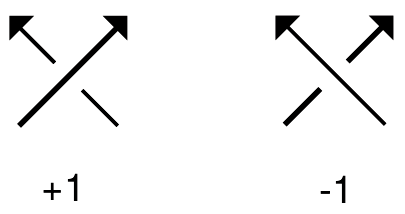
\includegraphics[width=5cm]{Images/linking_number.png}
		\end{center}\caption{Computando o \textit{linking number}}\label{linking number}
	\end{figure}
	\par\vspace{0.3cm} Contamos $+1$ se a seta "por cima" está à direita da seta "por baixo" e $-1$ se o contrário ocorre. Podemos ainda chamar $+1$ e $-1$ de cruzamentos destro e canhoto, respectivamente. Às vezes, pode ser um pouco difícil determinar qual o tipo de cruzamento a partir do diagrama. Uma dica é notar que para cruzamentos destros, podemos girar a seta inferior no sentido horário de forma que as duas setas coincidam; analogamente, para cruzamentos canhotos podemos girar a seta inferior no sentido anti-horário de forma que as duas seta coincidam.
	\par\vspace{0.3cm} Agora, vamos somar os $+1$ e $-1$ de todos os cruzamentos entre $M$ e $N$ e dividir essa soma por $2$. Esse é o \textit{linking number}. Note que nós não levamos em consideração para o cálculo do \textit{linking number} os autocruzamentos dos componentes $M$ e $N$. 
	\begin{figure}[H]
		\begin{center}
			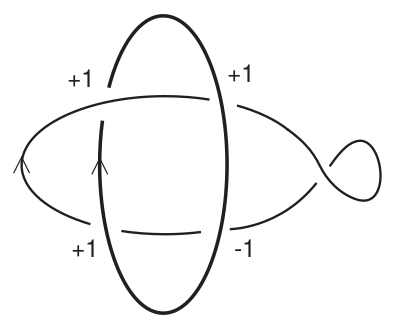
\includegraphics[width=5cm]{Images/exemplo_linking_number.png}
		\end{center}\caption{\textit{Linking number}$ = (1+1+1-1)/2 = 1$}\label{exemplo linking number}
	\end{figure}
	\par\vspace{0.3cm} Note, na Figura \eqref{exemplo linking number}, que se revertermos a orientação de apenas um dos dois componentes, o \textit{linking number} será multiplicado por $-1$. Contudo, se pensarmos no valor absoluto do \textit{linking number} então ele independe da orientação dada aos componentes.
	\par\vspace{0.3cm} Note que usamos uma projeção particular do \textit{link} para computar o \textit{linking number}. De fato, vamos mostrar que o \textit{linking number} independe da projeção escolhida. Para tal, vamos mostrar que os movimentos de Reidemeister não alteram o \textit{linking number}. Uma vez que podemos sair de uma projeção de um \textit{link} para qualquer outra projeção desse mesmo \textit{link} via uma sequência de movimentos de Reidemeister, então duas projeções do mesmo \textit{link} devem, necessariamente, nos dar o mesmo \textit{linking number}.
	\par\vspace{0.3cm} Vamos primeiro analisar o efeito de um movimento de Reidemeister tipo I, $\Omega_1$. Da Figura \eqref{reidemeister tipo 1}, vemos que esse movimento apenas introduz autocruzamentos, não afetando, portanto, o \textit{linking number}. Agora os movimentos tipo II e III, $\Omega_2$ e $\Omega_3$. Observe a figura a seguir.
	%
% 	\begin{figure}[H]
% 		\centering
% 		\begin{subfigure}[t]{0.5\textwidth}
% 			\centering
% 			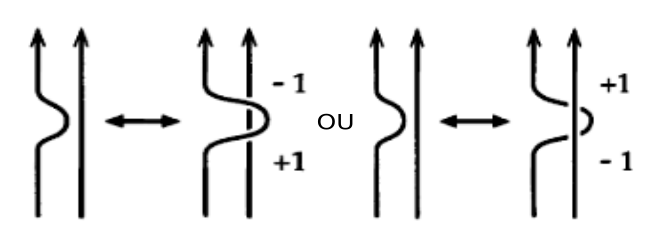
\includegraphics[width=6cm]{Images/reidemeister2linkingnumber.png}
% 			\caption{}
% 			\label{omega2}
% 		\end{subfigure}%
% 		~ 
% 		\begin{subfigure}[t]{0.5\textwidth}
% 			\centering
% 			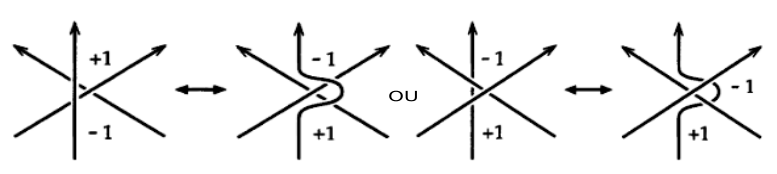
\includegraphics[width=7cm, height=2cm]{Images/reidemeister3linkingnumber.png}
% 			\caption{}
% 			\label{omega3}
% 		\end{subfigure}
% 		\caption{Os movimentos de Reidemeister tipo II e tipo III não alteram o \textit{linking number}.}
% 	\end{figure}
	%
	%
	\begin{figure}[H]
        \centering
        \subfloat[]{\label{omega2}{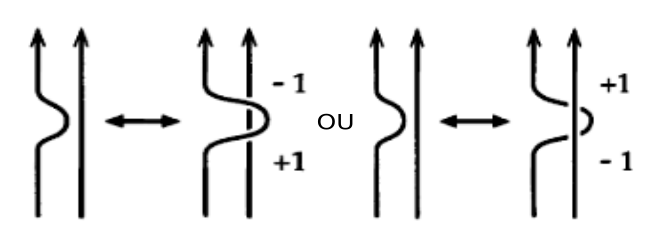
\includegraphics[width=6cm]{Images/reidemeister2linkingnumber.png}}}\hfill
        \subfloat[]{\label{omega3}{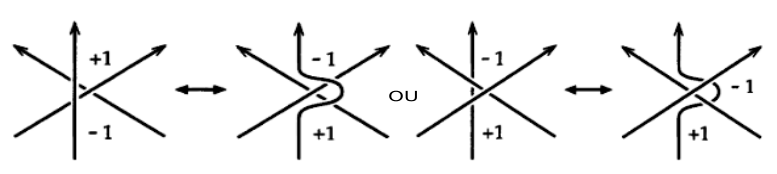
\includegraphics[width=7cm,height=2cm]{Images/reidemeister3linkingnumber.png}}}
        \caption{Os movimentos de Reidemeister tipo II e tipo III não alteram o \textit{linking number}}
    \end{figure}
	%
	\par\vspace{0.3cm} Portanto, os movimentos de Reidemeister de fato não alteram o \textit{linking number}. Daí, podemos dizer que o \textit{linking number} é um invariante de \textit{link} (orientado). Com isso, podemos usá-lo para distinguir \textit{links} (se quisermos distinguir \textit{links} não orientados, basta tomar o módulo do \textit{linking number}).
	
	\section{Tranças, nós e protetores solares de para-brisa}
	\hspace{12pt} Você já deve estar familiarizado com aqueles protetores solares de para-brisa, meio arredondados como na Figura \eqref{protetor solar}, que lembram um disco e que se dobram de maneira um tanto quanto estranha.
	
	\begin{figure}[H]
		\begin{center}
			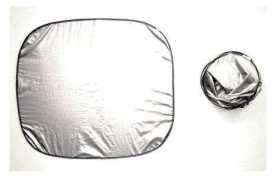
\includegraphics[width=6cm]{Images/protetor_solar.png}
		\end{center}\caption{O protetor de para-brisa aberto e fechado}\label{protetor solar}
	\end{figure}
	\par\vspace{0.3cm} Vamos analisar mais de perto a estrutura desse protetor de para-brisa. A parte fundamental do protetor é um arame metálico que percorre todo o perímetro do protetor, formando um \text{loop} contínuo. Esse arame é torcionalmente rígido, i.e., podemos dobrá-lo ao longo de seu comprimento sem problemas, mas não podemos torcê-lo. Esse fato servirá de base para a nossa análise.
	\par\vspace{0.3cm} Esse arame do protetor, quando aberto, tem a forma aproximada de um círculo, sem torções no arame. Quando fechado, esse arame deve ser enrolado em vários círculo/\textit{loops} menores, mas sem que haja torção do arame. Para ser mais preciso, perguntamos o seguinte:
	\begin{enumerate}
		\item Com o protetor na sua posição fechada "normal", quantos \textit{loops} o arame faz, e por quê?
		\item De modo mais geral, quais são todas as possíveis posições fechadas para o protetor, em termos de quantos \textit{loops} o arame faz? 
	\end{enumerate} 
	\par\vspace{0.3cm} Note que a parte de "quantos" da pergunta 1 pode ser respondida através de observações experimentais, dobrando o protetor de fato, mas isso não nos ajuda a responder a parte do "por quê".
	\par\vspace{0.3cm} Antes de prosseguir, um pouco de terminologia: vamos dizer que o arame é uma fita. Essa fita tem duas arestas, que chamaremos de círculos de fronteira. Vamos também chamar de centro o círculo no meio do caminho entre os círculos de fronteira. 
	\par\vspace{0.3cm} Agora, vamos esclarecer o que significa dizer que quando o protetor está fechado a fita é "enrolada" em vários \textit{loops}.
	\par\vspace{0.3cm} Informalmente, isso seria como enrolar um pedaço de linha em um carretel e depois juntar as pontas da linha (de forma que o pedaço de linha é ele próprio um \textit{loop}). De fato, isso é exatamente o que temos em mente; contudo, para sermos mais gerais, devemos permitir que essa linha passe por baixo dos \textit{loops} que já estão no carretel, e é aqui que entram as tranças! 
	\begin{figure}[H]
		\begin{center}
			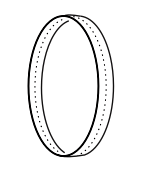
\includegraphics[width=3cm]{Images/fita.png}
		\end{center}\caption{O centro da fita (pontilhado) e os círculos de fronteira (curvas sólidas) com o protetor aberto.}
	\end{figure}
	\par\vspace{0.3cm} A partir da maneira que estamos considerando o protetor e do que dissemos acima, podemos ver que o seguinte é verdade:
	\begin{center}
		\textbf{Afirmação 1. Com o protetor fechado, o centro da fita é uma trança fechada de um componente, ou seja, um nó.}
	\end{center}
	\par\vspace{0.3cm} Então, suponha que nossa trança fechada de um componente foi construída a partir de uma trança de $m$ cordas e com $n$ cruzamentos. Como nossa trança fechada tem apenas um componente, temos que $m$ e $n$ têm paridades diferentes.
	\par\vspace{0.3cm} Isso se deve ao fato de que a permutação associada à nossa trança fechada deve ter a forma
	\begin{equation*}
	(i_1i_2\cdots i_m) = \underbrace{(i_1i_m)(i_1i_{m-1})\cdots(i_1i_2)}_{m-1\text{ transposições}}
	\end{equation*}
	\par\vspace{0.3cm} sendo que cada $i_j$ é um elemento distinto do conjunto $\left\{1, 2, \dots, m \right\}$. Consequentemente, como $m-1=n$, segue que $m$ e $n$ têm paridades distintas. Daí, sabemos também que o seguinte é verdade:
	\begin{center}
		\textbf{Afirmaação 2. Com o protetor fechado, se a fita é enrolada em m \textit{loops} e o centro da fita tem n cruzamentos, então m e n têm paridades opostas.}
	\end{center}
	\par\vspace{0.3cm} Agora vamos considerar os dois círculos de fronteira da fita. Aqui entram os \textit{links} e o \textit{linking number}!
	\par\vspace{0.3cm} Nessa análise, o que nos interessa é o fato de que o valor absoluto do \textit{linking number} é um invariante topológico.
	\par\vspace{0.3cm} Com o protetor aberto, o \textit{linking number} dos círculos de fronteira é, claramente, $0$. Como esse valor não muda quando dobramos o protetor, o seguinte também é verdade:
	\begin{center}
		\textbf{Afirmação 3. Com o protetor fechado, o \textit{linking number} dos círculos de fronteira é 0.}
	\end{center}
	\par\vspace{0.3cm} Agora, pense no protetor fechado. Como a fita não tem torções, os únicos cruzamentos entre os círculos de fronteira ocorrem próximo dos $n$ autocruzamentos do centro, como na Figura \eqref{cruzamentos protetor}. O centro da fita já serviu seu próposito; podemos ignorá-lo agora. Agora, no lugar dos $n$ autocruzamentos do centro, vemos $4$ novos cruzamentos envolvendo os círculos de fronteira: dois autocruzamentos e dois cruzamentos. Como estamos interessados no \textit{linking number} dos círculos de fronteira, vamos ignorar os autocruzamentos. Então, temos um total de $2n$ cruzamentos, arranjados em $n$ pares, entre os círculos de fronteira.
	
	\begin{figure}[H]
		\begin{center}
			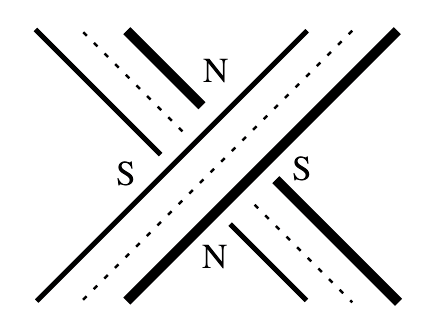
\includegraphics[width=4.5cm]{Images/protetor_fechado.png}
		\end{center}\caption{A letra $S$ indica os autocruzamentos dos círculos de fronteira e $N$ indica os outros cruzamentos. A linha contínua mais grossa indica um dos círculos de fronteira, enquanto que a linha contínua mais fina indica o outro. A linha pontilhada representa o centro da fita.}\label{cruzamentos protetor}
	\end{figure}
	\par\vspace{0.3cm} Para computar o \textit{linking number}, olhe novamente para a Figura \eqref{cruzamentos protetor} e note que para cada círculo de fronteira, seus dois pedaços na figura estarão orientados ambos para cima ou para baixo. Daí, segue que em cada um dos $n$ pares de cruzamentos temos ou dois $+1$ (círculos orientados para cima) ou dois $-1$ (círculos orientados para baixo). Portanto, cada um desses $n$ pares de cruzamentos contribui com exatamente $1$ ou $-1$ para o \textit{linking number}.
	\par\vspace{0.3cm} Note que $1$ e $-1$ são ambos ímpares, e se somarmos $n$ números ímpares o resultado tem a mesma paridade de $n$. Mas, pela Afirmação 3, o \textit{linking number} é $0$; logo, $n$ deve ser par. Portanto, pela Afirmação 2, $m$ deve ser ímpar e demonstramos o teorema:
	\begin{theorem}
		\label{teorema protetor de para-brisa}
		Quando fechado, o arame do protetor deve ser enrolado em um número ímpar de \textit{loops}.
	\end{theorem}  
	\par\vspace{0.3cm} De fato, o arame do protetor se enrola em 3 \textit{loops} (respondendo à pergunta 1) não havendo torsões no arame. Para responder à pergunta 2, você pode verificar experimentalmente que mesmo sendo possível forçar o protetor em 2 ou 4 \textit{loops}, isso causará torsões no arame. Contudo, $3$ \textit{loops} não é a única configuração possível, como demonstramos: em tese, qualquer número ímpar de \textit{loops} pode ser alcançado.